\documentclass[a4paper]{article}
\usepackage[a4paper,top=2cm,bottom=2cm,left=1cm,right=1cm,marginparwidth=1.75cm]{geometry}
% \usepackage[spanish]{babel}
% \selectlanguage{spanish}
% \usepackage[utf8]{inputenc}
% \usepackage[T1]{fontenc}
% \usepackage[spanish]{babel}

% \usepackage[T1]{fontenc}
\usepackage{graphicx} %Paquete para usar imagenes
\usepackage{listings}
\usepackage{xcolor}
\usepackage{tcolorbox}\usepackage{hyperref}

\definecolor{background}{HTML}{E7EBF4}
\definecolor{bg}{HTML}{1a1b26}
\definecolor{fg}{HTML}{a9b1d6}
\definecolor{comment}{HTML}{848cb5}
\definecolor{cyan}{HTML}{82aaff}
\definecolor{orange}{HTML}{ff9e64}
\definecolor{yellow}{HTML}{e9d78e}
\definecolor{purple}{HTML}{c792ea}
\definecolor{green}{HTML}{7fdbca}
\definecolor{numbers}{HTML}{9854f1}
\definecolor{keyword}{HTML}{9854f1}

\lstset{
    showspaces=false, % Evita mostrar espacios en blanco como ␣
    showstringspaces=false,
    inputencoding=utf8,
    extendedchars=true,
    literate=%
    {á}{{\'a}}1
    {é}{{\'e}}1
    {í}{{\'i}}1
    {ó}{{\'o}}1
    {ú}{{\'u}}1
    {ñ}{{\~n}}1
}
\lstdefinestyle{mystyle}{
    language=Python,
    basicstyle=\ttfamily,
    keywordstyle=\color{keyword},
    commentstyle=\color{comment},
    numbers=none,
    numberstyle=\tiny\color{numbers},
    frame=none,
    breaklines=true,
    % showstringspaces=false
    xleftmargin=0mm,
    xrightmargin=0mm,
}

\lstset{style=mystyle}

\newtcolorbox{mycodebox}[1][]{
    arc=17pt,  % Radio de las esquinas redondeadas
    colback=background,  % Color de fondo del cuadro
    boxrule=0.5pt,  % Grosor de la línea del cuadro
    colframe=background,
    width=0.8\textwidth,   % Anchura del cuadro
    % height=5cm,            % Altura del cuadro
    % breakable,
    #1  % Otras opciones personalizadas que puedas necesitar
}


\newtcolorbox{mycodeboxl}[1][]{
    arc=7pt,  % Radio de las esquinas redondeadas
    colback=background,  % Color de fondo del cuadro
    boxrule=0.5pt,  % Grosor de la línea del cuadro
    colframe=background,
    width=0.94\textwidth,   % Anchura del cuadro
    % height=5cm,            % Altura del cuadro
    % breakable,
    #1  % Otras opciones personalizadas que puedas necesitar
}

% Documento
\begin{document}
\newgeometry{left=3cm,right=3cm,top=2cm,bottom=2cm}
\begin{titlepage}

%--------------- Nuevo comendo de linea ----------------->
\newcommand{\linea}{\rule{\linewidth}{0.7mm}} 
\center
%--------------- Universidad, facultad y carrera ----------------->
\textbf{\Large UNIVERSIDAD NACIONAL DE SAN ANTONIO ABAD DEL CUSCO}\\[0.2cm]
\textbf{\Large FACULTAD DE INGENIERÍA ELÉCTRICA, ELECTRÓNICA,INFORMÁTICA Y MECÁNICA}\\[0.2cm]
\textbf{\Large INGENIERÍA INFORMÁTICA Y DE SISTEMAS\\[0.6cm]}

%--------------- Escudos png ----------------->

\includegraphics[width=8cm]{src/escudo-unsaac.png}
\vfill

%--------------- Tema ----------------->
\linea
\\[0.3cm]
% \vfill
\textbf{\LARGE Guía de Laboratorio 9 - Transformaciones en el espacio 3D}\\[0.2cm]
\linea \\
\vfill

%--------------- Integrantes ----------------->
\textit{\Large Alumno:}\\
%Integrantes del grupo
    \textbf{\large Ian Logan Will Quispe Ventura}\\
    \textit{211359}\\
    % \vfill

%--------------- Profesor y curso ----------------->
\vspace{0.3cm}
    \textit{\Large Docente:}\\
    \textbf{\large Hector Eduardo Ugarte Rojas}\\
\vspace{0.5cm}
    \textit{\Large Curso:}\\
    \textbf{\large Computación Gráfica}\\
    \vfill

\vspace{0.4cm}
    \textbf{\Large Cusco - Perú }\\
    \textbf{\large 2023 - II }\\
    \newpage
    \end{titlepage}

\restoregeometry
\newpage
% •·•·•·•·•·•••·•·•·•·•·•·•·•·•·•·•·•·•·•·•·•·•·•·•·•·•.,..,
% \section{Funcionamiento del algoritmo DDA}

\Large{\textbf{Traslación de una piramide}}\\[-0.4cm]
\begin{center}
\begin{mycodeboxl}
\begin{lstlisting}
from OpenGL.GL import *
from OpenGL.GLUT import *
import numpy as np

WIDTH, HEIGHT = 400, 400
C = np.zeros((4, 1))

def multiplicacion(A, FA, CA, B, FB, CB, C):
    if CA == FB:
        for i in range(FA):
            for j in range(CB):
                C[i][j] = 0
                for k in range(CA):
                    C[i][j] += A[i][k] * B[k][j]

def ejes():
    glBegin(GL_LINES)
    glColor3f (0.4 , 0.4 , 0.3) # Color3
    glVertex3i(0, 0, 0)  # eje Y
    glVertex3i(0, 50, 0)
    glVertex3i(0, 0, 0)  # eje X
    glVertex3i(50, 0, 0)
    glVertex3i(0, 0, 0)  # eje Z
    glVertex3i(0, 0, 50)
    glEnd()

def display():
    glClear(GL_COLOR_BUFFER_BIT | GL_DEPTH_BUFFER_BIT)
    glColor3f(0.5 , 0.3 , 0.9)  
    ejes()
    glColor3f(0.8, 0.26, 1.0)  # color 
    A1 = np.array([[0.0], [0.0], [0.0], [1.0]])
    B1 = np.array([[10.0], [0.0], [0.0], [1.0]])
    C1 = np.array([[0.0], [10.0], [0.0], [1.0]])
    D1 = np.array([[0.0], [0.0], [10.0], [1.0]])
\end{lstlisting}
\end{mycodeboxl}
\end{center}
% -------------------------------------------------------------------
\newpage
\begin{center}
\begin{mycodeboxl}
\begin{lstlisting}
    glPolygonMode(GL_FRONT_AND_BACK, GL_LINE)
    glBegin(GL_TRIANGLE_STRIP)
    glVertex3f(A1[0][0], A1[1][0], A1[2][0])
    glVertex3f(B1[0][0], B1[1][0], B1[2][0])
    glVertex3f(C1[0][0], C1[1][0], C1[2][0])
    glVertex3f(D1[0][0], D1[1][0], D1[2][0])
    glVertex3f(A1[0][0], A1[1][0], A1[2][0])
    glEnd()

    t = np.array([10, -8, 8])
    T = np.array([[1.0, 0.0, 0.0, t[0]],
                  [0.0, 1.0, 0.0, t[1]],
                  [0.0, 0.0, 1.0, t[2]],
                  [0.0, 0.0, 0.0, 1.0]])

    multiplicacion(T, 4, 4, A1, 4, 1, C)
    A2 = C.copy()
    multiplicacion(T, 4, 4, B1, 4, 1, C)
    B2 = C.copy()
    multiplicacion(T, 4, 4, C1, 4, 1, C)
    C2 = C.copy()
    multiplicacion(T, 4, 4, D1, 4, 1, C)
    D2 = C.copy()

    glColor3f(0.0, 1.0, 0.0)  # color 
    glPolygonMode(GL_FRONT_AND_BACK, GL_LINE)
    glBegin(GL_TRIANGLE_STRIP)
    glVertex3f(A2[0][0], A2[1][0], A2[2][0])
    glVertex3f(B2[0][0], B2[1][0], B2[2][0])
    glVertex3f(C2[0][0], C2[1][0], C2[2][0])
    glVertex3f(D2[0][0], D2[1][0], D2[2][0])
    glVertex3f(A2[0][0], A2[1][0], A2[2][0])
    glEnd()

    glutSwapBuffers()
\end{lstlisting}
\end{mycodeboxl}
\end{center}

\begin{center}
\begin{mycodebox}
\begin{lstlisting}

def ini():
    glClearColor (0.9 ,0.92 , 0.95 , 1.0) # Fondo
    glMatrixMode(GL_PROJECTION)
    glLoadIdentity()
    glOrtho(-18.0, 30.0, -15.0, 30.0, -30.0, 30.0)
    glMatrixMode(GL_MODELVIEW)
    glLoadIdentity()
    glRotatef(90.0, 3.0, 3.0, 3.0)

def main():
    glutInit()
    glutInitDisplayMode(GLUT_DOUBLE | GLUT_RGB | GLUT_DEPTH)
    glutInitWindowSize(WIDTH, HEIGHT)
    glutInitWindowPosition(0, 0)
    glutCreateWindow("Traslación 3D")
    glutDisplayFunc(display)
    ini()
    glutMainLoop()

if __name__ == "__main__":
    main()
\end{lstlisting}
\end{mycodebox}
\end{center}

\newpage
Gráfico generado 
\begin{center}
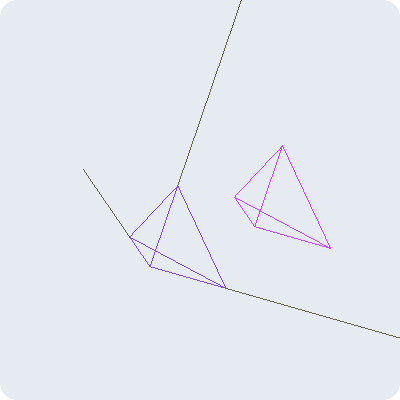
\includegraphics[width=16cm]{./src/1.png}
\end{center}
% -------------------------------------------------------------------
\newpage
\Large{\textbf{Rotación general de un piramide}}\\[-0.4cm]
\begin{center}
\begin{mycodeboxl}
\begin{lstlisting}
from OpenGL.GL import *
from OpenGL.GLUT import *
import numpy as np

WIDTH, HEIGHT = 400, 400
C = np.zeros((4, 1))

def multiplicacion(A, FA, CA, B, FB, CB, C):
    if CA == FB:
        for i in range(FA):
            for j in range(CB):
                C[i][j] = 0
                for k in range(CA):
                    C[i][j] += A[i][k] * B[k][j]
def ejes():
    glBegin(GL_LINES)
    glVertex3i(0, 0, 0)  # eje Y
    glVertex3i(0, 50, 0)
    glVertex3i(0, 0, 0)  # eje X
    glVertex3i(50, 0, 0)
    glVertex3i(0, 0, 0)  # eje Z
    glVertex3i(0, 0, 50)
    glEnd()

def display():
    glClear(GL_COLOR_BUFFER_BIT | GL_DEPTH_BUFFER_BIT)

    glColor3f(1.0, 1.0, 0.0)  # color amarillo
    ejes()

    glColor3f(1.0, 0.0, 0.0)  # color 
    A1 = np.array([[0.0], [0.0], [0.0], [1.0]])
    B1 = np.array([[20.0], [0.0], [0.0], [1.0]])
    C1 = np.array([[0.0], [20.0], [0.0], [1.0]])
    D1 = np.array([[0.0], [0.0], [20.0], [1.0]])
\end{lstlisting}
\end{mycodeboxl}
\end{center}
% -------------------------------------------------------------------
\newpage
\begin{center}
\begin{mycodeboxl}
\begin{lstlisting}
    glPolygonMode(GL_FRONT_AND_BACK, GL_LINE)
    glBegin(GL_TRIANGLE_STRIP)
    glVertex3f(A1[0][0], A1[1][0], A1[2][0])
    glVertex3f(B1[0][0], B1[1][0], B1[2][0])
    glVertex3f(C1[0][0], C1[1][0], C1[2][0])
    glVertex3f(D1[0][0], D1[1][0], D1[2][0])
    glVertex3f(A1[0][0], A1[1][0], A1[2][0])
    glEnd()

    # Rotar a través de un ángulo de 45 grados alrededor
    # de la línea que pasa por C1 en la dirección [0, 1, 1]
    T = np.array([[0.7071, -0.5, 0.5, 0.5],
                  [0.5, 0.8536, 0.1464, 0.1464],
                  [-0.5, 0.1464, 0.8536, -0.1464],
                  [0, 0, 0, 1]])

    multiplicacion(T, 4, 4, A1, 4, 1, C)
    A2 = C.copy()
    multiplicacion(T, 4, 4, B1, 4, 1, C)
    B2 = C.copy()
    multiplicacion(T, 4, 4, C1, 4, 1, C)
    C2 = C.copy()
    multiplicacion(T, 4, 4, D1, 4, 1, C)
    D2 = C.copy()

    glColor3f(0.0, 1.0, 0.0)  # color 
    glPolygonMode(GL_FRONT_AND_BACK, GL_LINE)
    glBegin(GL_TRIANGLE_STRIP)
    glVertex3f(A2[0][0], A2[1][0], A2[2][0])
    glVertex3f(B2[0][0], B2[1][0], B2[2][0])
    glVertex3f(C2[0][0], C2[1][0], C2[2][0])
    glVertex3f(D2[0][0], D2[1][0], D2[2][0])
    glVertex3f(A2[0][0], A2[1][0], A2[2][0])
    glEnd()

    glutSwapBuffers()
\end{lstlisting}
\end{mycodeboxl}
\end{center}

\begin{center}
\begin{mycodeboxl}
\begin{lstlisting}
def ini():
    glClearColor(0.0, 0.0, 0.0, 1.0)
    glMatrixMode(GL_PROJECTION)
    glLoadIdentity()
    glOrtho(-50.0, 50.0, -50.0, 50.0, -50.0, 50.0)
    glMatrixMode(GL_MODELVIEW)
    glLoadIdentity()
    glRotatef(45.0, 3.0, 3.0, 3.0)

def main():
    glutInit()
    glutInitDisplayMode(GLUT_DOUBLE | GLUT_RGB | GLUT_DEPTH)
    glutInitWindowSize(WIDTH, HEIGHT)
    glutInitWindowPosition(0, 0)
    glutCreateWindow("Rotación 3D")
    glutDisplayFunc(display)
    ini()
    glutMainLoop()

if __name__ == "__main__":
    main()
\end{lstlisting}
\end{mycodeboxl}
\end{center}


\newpage
Gráfico generado 
\begin{center}
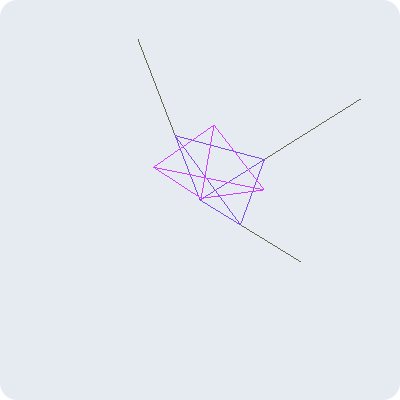
\includegraphics[width=16cm]{./src/2.png}
\end{center}

\newpage
% -------------------------------------------------------------------
\Large{\textbf{Rotación de un cubo en 30° por una linea arbitraria}}\\[-0.4cm]
\begin{center}
\begin{mycodeboxl}
\begin{lstlisting}
from OpenGL.GL import *
from OpenGL.GLUT import *
from OpenGL.GLU import gluPerspective, gluLookAt
import numpy as np

ANCHO, ALTO = 400, 400

def rotar_alrededor_del_eje(vertices, eje, angulo):
    angulo_radianes = np.radians(angulo)
    cos_theta = np.cos(angulo_radianes)
    sin_theta = np.sin(angulo_radianes)

    eje = np.array(eje, dtype=np.float64)
    eje /= np.linalg.norm(eje)

    vertices_rotados = []
    for face in vertices:
        rotated_face = []
        for vertex in face:
            vertex = np.array(vertex)
            u = eje[0]
            v = eje[1]
            w = eje[2]
            
            x_rot = (u * (u * vertex[0] + v * vertex[1] + w * vertex[2]) * (1 - cos_theta) +
                     vertex[0] * cos_theta + (-w * vertex[1] + v * vertex[2]) * sin_theta)
            
            y_rot = (v * (u * vertex[0] + v * vertex[1] + w * vertex[2]) * (1 - cos_theta) +
                     vertex[1] * cos_theta + (w * vertex[0] - u * vertex[2]) * sin_theta)
\end{lstlisting}
\end{mycodeboxl}
\end{center}
\begin{center}
\begin{mycodeboxl}
\begin{lstlisting}
            z_rot = (w * (u * vertex[0] + v * vertex[1] + w * vertex[2]) * (1 - cos_theta) +
                     vertex[2] * cos_theta + (-v * vertex[0] + u * vertex[1]) * sin_theta)
            
            rotated_face.append([x_rot, y_rot, z_rot])

        vertices_rotados.append(rotated_face)

    return vertices_rotados

def dibujar_cubo(vertices, color):
    glColor3fv(color)
    glPolygonMode(GL_FRONT_AND_BACK, GL_LINE)
    glBegin(GL_QUADS)
    for face in vertices:
        for vertex in face:
            glVertex3fv(vertex)
    glEnd()

def ejes():
    glBegin(GL_LINES)
    glColor3f (0.4 , 0.4 , 0.3) # Color3
    glVertex3i(0, 0, 0)  # eje Y
    glVertex3i(0, 50, 0)
    glVertex3i(0, 0, 0)  # eje X
    glVertex3i(50, 0, 0)
    glVertex3i(0, 0, 0)  # eje Z
    glVertex3i(0, 0, 50)
    glEnd()
\end{lstlisting}
\end{mycodeboxl}
\end{center}
\begin{center}
\begin{mycodeboxl}
\begin{lstlisting}
def display():
    glClear(GL_COLOR_BUFFER_BIT | GL_DEPTH_BUFFER_BIT)
    ejes()
    A1 = [-10.0, -10.0, -10.0]
    B1 = [10.0, -10.0, -10.0]
    C1 = [10.0, 10.0, -10.0]
    D1 = [-10.0, 10.0, -10.0]
    E1 = [-10.0, -10.0, 10.0]
    F1 = [10.0, -10.0, 10.0]
    G1 = [10.0, 10.0, 10.0]
    H1 = [-10.0, 10.0, 10.0]

    vertices = [[A1, B1, C1, D1],
        [E1, F1, G1, H1],
        [A1, B1, F1, E1],
        [D1, C1, G1, H1],
        [B1, F1, G1, C1],
        [A1, E1, H1, D1]]

    # Dibuja el cubo original 
    dibujar_cubo(vertices,[0.5 , 0.3 , 0.9])
    # Aplica rotación alrededor de [7, 7, 7] con un ángulo de 30 grados
    vertices_rotados = rotar_alrededor_del_eje(vertices, [7, 7, 7], 30)
    dibujar_cubo(vertices_rotados, [0.8, 0.26, 1.0])
    glutSwapBuffers()

def inicializar():
    glClearColor (0.9 ,0.92 , 0.95 , 1.0) # Fondo
    glMatrixMode(GL_PROJECTION)
    glLoadIdentity()
    glOrtho(-3.0, 2.0, -3.0, 2.0, -2.0, 2.0)
    gluPerspective(45.0, float(ANCHO) / float(ALTO), 1, 100.0)
    glMatrixMode(GL_MODELVIEW)
    glLoadIdentity()
    gluLookAt(25, 25, 50, 25, 25, 0, 0, 1, 0)
\end{lstlisting}
\end{mycodeboxl}
\end{center}


\begin{center}
\begin{mycodeboxl}
\begin{lstlisting}
def main():
    glutInit()
    glutInitDisplayMode(GLUT_DOUBLE | GLUT_RGB | GLUT_DEPTH)
    glutInitWindowSize(ANCHO, ALTO)
    glutInitWindowPosition(0, 0)
    glutCreateWindow("Rotación 3D")
    glutDisplayFunc(display)
    inicializar()
    glEnable(GL_DEPTH_TEST)
    glutMainLoop()

if __name__ == "__main__":
    main()
\end{lstlisting}
\end{mycodeboxl}
\end{center}

Gráfico generado 
\begin{center}

\includegraphics[width=14cm]{./src/3.png}
\end{center}
\newpage
% -------------------------------------------------------------------
\Large{\textbf{Rotar un tetahedro en 45° respecto a una linea que pasa por [2,1,0] y [6,5,0]}}\\[-0.4cm]
\begin{center}
\begin{mycodeboxl}
\begin{lstlisting}
from OpenGL.GL import *
from OpenGL.GLUT import *
from OpenGL.GLU import gluPerspective, gluLookAt
import numpy as np

ANCHO, ALTO = 400, 400

def rotar_alrededor_del_eje(vertices, eje, angulo):
    angulo_radianes = np.radians(angulo)
    cos_theta = np.cos(angulo_radianes)
    sin_theta = np.sin(angulo_radianes)

    eje = np.array(eje, dtype=np.float64)
    eje /= np.linalg.norm(eje)

    vertices_rotados = []
    for vertex in vertices:
        u, v, w = eje
        x_rot = (u * (u * vertex[0] + v * vertex[1] + w * vertex[2]) * (1 - cos_theta) +
                 vertex[0] * cos_theta + (-w * vertex[1] + v * vertex[2]) * sin_theta)
        
        y_rot = (v * (u * vertex[0] + v * vertex[1] + w * vertex[2]) * (1 - cos_theta) +
                 vertex[1] * cos_theta + (w * vertex[0] - u * vertex[2]) * sin_theta)

        z_rot = (w * (u * vertex[0] + v * vertex[1] + w * vertex[2]) * (1 - cos_theta) +
                 vertex[2] * cos_theta + (-v * vertex[0] + u * vertex[1]) * sin_theta)
        
        vertices_rotados.append([x_rot, y_rot, z_rot])

    return vertices_rotados
\end{lstlisting}
\end{mycodeboxl}
\end{center}

\begin{center}
\begin{mycodeboxl}
\begin{lstlisting}

def dibujar_tetraedro(vertices, color):
    glColor3fv(color)
    glPolygonMode(GL_FRONT_AND_BACK, GL_LINE)
    glBegin(GL_TRIANGLES)
    glVertex3fv(vertices[0])  # Triángulo ABC
    glVertex3fv(vertices[1])
    glVertex3fv(vertices[2])
    glEnd()
    glBegin(GL_TRIANGLES)
    glVertex3fv(vertices[0])  # Triángulo ABD
    glVertex3fv(vertices[1])
    glVertex3fv(vertices[3])
    glEnd()
    glBegin(GL_TRIANGLES)
    glVertex3fv(vertices[0])  # Triángulo ACD
    glVertex3fv(vertices[2])
    glVertex3fv(vertices[3])
    glEnd()
    glBegin(GL_TRIANGLES)
    glVertex3fv(vertices[1])  # Triángulo BCD
    glVertex3fv(vertices[2])
    glVertex3fv(vertices[3])
    glEnd()

def ejes():
    glBegin(GL_LINES)
    glColor3f (0.4 , 0.4 , 0.3) # Color3
    glVertex3i(0, 0, 0)  # eje Y
    glVertex3i(0, 50, 0)
    glVertex3i(0, 0, 0)  # eje X
    glVertex3i(50, 0, 0)
    glVertex3i(0, 0, 0)  # eje Z
    glVertex3i(0, 0, 50)
    glEnd()
\end{lstlisting}
\end{mycodeboxl}
\end{center}

\begin{center}
\begin{mycodeboxl}
\begin{lstlisting}

def display():
    glClear(GL_COLOR_BUFFER_BIT | GL_DEPTH_BUFFER_BIT)

    ejes()

    A = [0.0, 10.0, 0.0]
    B = [10.0, -10.0, 0.0]
    C = [-10.0, -10.0, 0.0]
    D = [0.0, 0.0, 10.0]

    vertices = [A, B, C, D]

    # Dibuja el tetraedro original en color azul
    dibujar_tetraedro(vertices, [0.5 , 0.3 , 0.9])

    # Aplica rotación alrededor de [4, 4, 0] con un ángulo de 45 grados
    vertices_rotados = rotar_alrededor_del_eje(vertices, [4, 4, 0], 45)
    dibujar_tetraedro(vertices_rotados, [0.8, 0.26, 1.0])

    glutSwapBuffers()

def inicializar():
    glClearColor (0.9 ,0.92 , 0.95 , 1.0) # Fondo
    glMatrixMode(GL_PROJECTION)
    glLoadIdentity()
    glOrtho(-2.0, 2.0, -2.0, 2.0, -2.0, 2.0)
    gluPerspective(45.0, float(ANCHO) / float(ALTO), 1, 100.0)
    glMatrixMode(GL_MODELVIEW)
    glLoadIdentity()
    gluLookAt(30, 30, 30, 0, 0, 0, 0, 1, 0)
\end{lstlisting}
\end{mycodeboxl}
\end{center}

\begin{center}
\begin{mycodebox}
\begin{lstlisting}
def main():
    glutInit()
    glutInitDisplayMode(GLUT_DOUBLE | GLUT_RGB | GLUT_DEPTH)
    glutInitWindowSize(ANCHO, ALTO)
    glutInitWindowPosition(0, 0)
    glutCreateWindow("Rotación 3D")
    glutDisplayFunc(display)
    inicializar()
    glEnable(GL_DEPTH_TEST)
    glutMainLoop()

if __name__ == "__main__":
    main()
\end{lstlisting}
\end{mycodebox}
\end{center}

Gráfico generado 
\begin{center}
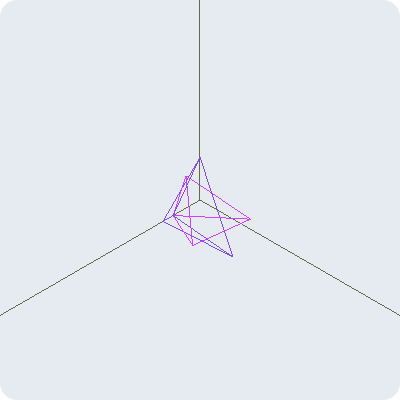
\includegraphics[width=14cm]{./src/4.png}
\end{center}
\newpage
% -------------------------------------------------------------------
\end{document}
